\chapter{Solution} \label{cha:solution}
This chapter is focused on the integration of the three modules of this thesis: detection, recognition and tracking. The explanation is based on the flow of the code, with special attention at the choices done and implementation details. The source code of the entire project is available on github\cite{projectSourceCode}.

\section{Wrapper function: follow} \label{sec:follow}
The code is entirely managed with a single class called \textbf{Follower}. This structure only requires to be initialized and then calling a "\textit{follow}" method (\Cref{alg:follow}) every time a new frame needs to be processed.\\
The class internally loads a new frame \li{2} from the webcam or, optionally, from a stored video. Both the sources can be used in "real-time". In fact, if the video is used some frames are internally discarded to simulate the losing of images due to a slow processing rate. Therefore the class \textit{Follower} can be analysed with both real-time tests but also recorded experiments. This feature is useful to replicate scenarios where the code have failed.\\
\\
The wrapper method \textit{follow} has only one task. It measures the elapsed time from the beginning of the tracking \li{4} and, according to this parameter, the \textit{slow start} phase (\Cref{sec:slowStartPhase}) is executed \li{5}  if less than X seconds are gone. Otherwise, the \textit{track leader} phase (\Cref{sec:trackleaderPhase}) is called \li{7}.

\begin{lstlisting}[captionpos=b, 
	caption={It is the pseudocode of the wrapper function that should grab the new incoming frames and redirect them to the first or second phase according to the time elapsed from the tracking begin.}, 
	label=alg:follow
	]
follow() -> position:
	frame = grab_newFrame()
	
	if elapsedTime() > phase1_length: #phase 1
	%*$\lfloor$*)	position = slowStartPhase(frame)
	else:							  #phase 2
	%*$\lfloor$*)	position = followPhase(frame)

	return position
\end{lstlisting}


\section{First phase: slow start} \label{sec:slowStartPhase}
This function is a novelty that we have chosen to introduce to empower the performances of the overall algorithm. The pseudo code of this method is provided at~\Cref{alg:slowStartPhase} while an example is shown in~\Cref{fig:slowStart}.\\
This project, differently from the traditional trackers and similarly to TLD (\Cref{sec:tld}), is based on an online learning classifier. Hence this phase is designed to immediately train KNN a little bit. This first generated knowledge will be then increased in the \textit{track leader} phase. KNN can classify the representative points that come from the bounding boxes of people in new frames, only according to other representative points previously archived. The \textit{slow start} phase is used to collect all the bounding boxes used to create the set of positive representative points into the N-dimensional space of KNN.\\
This elaboration works based on the assumption that during this first phase "\ul{The leader is the most important visible person}". The \textit{slow start} computes the detection of the visible people \li{3} and if one or more exists\li{5}, the leader is chosen as the bounding box, with the biggest area\li{6}. The X and Y pixel coordinates are computed to be retrieved \li{7} and the leader's box is given to KNN \li{8}. Simultaneously, a negative sample is randomly picked up from a database and it is also given to KNN \li{9}. This double fed is done to train KNN with a balanced number of positive and negative samples, in order to exploit the potentialities shown in~\Cref{fig:knn_googleNet_s9n18}. The negative samples come from a custom version of the Market1501 dataset\cite{market1501}, called \textbf{NegativePeople}, that we have created ad hoc for this purpose.\\
\\
The \textit{slow start} phase is executed for a period that can last for 3 up to 20 seconds or more. The value of this hyper-parameter influence the size of samples known by KNN when the official track starts. The longer this phase the better. The default value is set to 5 seconds. Alternatively, another possibility is that the first phase can be interrupted after that X points are given to KNN, but this does not guarantee a precise slot of time so this variant was discarded.

\begin{lstlisting}[captionpos=b, 
	caption={It is the pseudocode of the first phase. The function \textit{slow start} computes only detections in order to train the KNN people classifier.}, 
	label=alg:slowStartPhase
	]
slowStartPhase(frame) -> position:
	position = default
	boxes = detector.detectPeople(frame)
	
	if len(boxes)>=1:
	%*$\mid$*)	box = biggestAreaBB(boxes)
	%*$\mid$*)	position = getPosition(box)
	%*$\mid$*)	knn.addPositive(box)
	%*$\lfloor$*)	knn.addNegative(pickOneNegative())
	
	return position
\end{lstlisting}
\begin{figure}
	\centering
	\begin{minipage}{.49\textwidth}
		\centering
		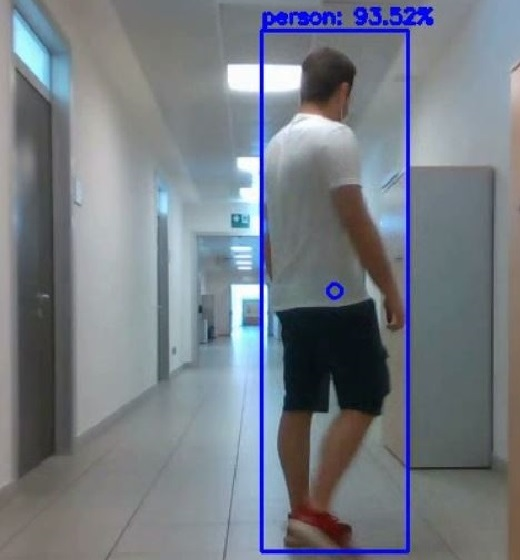
\includegraphics[width=1\linewidth]{images/solution/slowStart}
		\captionsetup{margin=0.2cm}
		\captionof{figure}[Frame of the slow start phase.]{Frame of the \textit{slow start} phase where the detection only is working. The leader has a \textbf{\textcolor{blue}{blue}} rectangle, and eventually other people are in \textbf{\textcolor{gray}{gray}}.}
		\label{fig:slowStart}
	\end{minipage}
	\begin{minipage}{.49\textwidth}
		\centering
		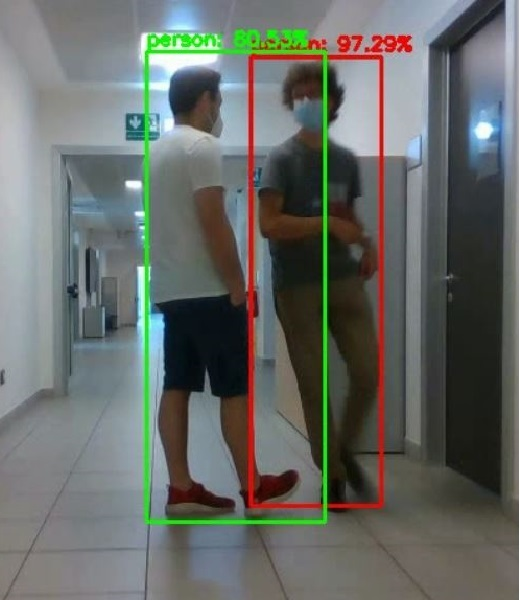
\includegraphics[width=1\linewidth]{images/solution/leaderSubjectOk}
		\captionsetup{margin=0.2cm}
		\captionof{figure}[A perfect detection example.]{A perfect detection where the two people are correctly recognised as leader (positive=\textbf{\textcolor{green}{green}}) and random person (negative=\textbf{\textcolor{red}{red}}).}
		\label{fig:doubleDetectionOk}
	\end{minipage}
\end{figure}


\section{Second phase: track leader} \label{sec:trackleaderPhase}
This function is the core of the entire project. The overall scheme of the pseudocode is shown at~\Cref{alg:trackleaderPhase}. In addition, in~\Cref{fig:sequenceTracking} there is a sequence of frames taken from a video clip where the robot is following the leader while it is shortly occluded twice by another person.\\
This phase works as follows:\\
\begin{itemize}
	\item The detection is performed \li{7} only one time every X frames \li{5}(details in~\Cref{sec:ratioDetectTrack}) and if the position of the leader is unknown \li{6}.\\
	The position is unknown immediately after the \textit{slow start} phase \li{2}, after the end of the tracking \li{29} and after a failed detection \li{17}.\\
	A sample detection over two people is shown in~\Cref{fig:doubleDetectionOk}.
	
	\item All the detections are elaborated \li{10} to check if are close to the last known position \li{11} and so can be kept or not (the drift optimization details are in~\Cref{sec:driftOptimization}). In addition, the KNN classifier is used \li{12} to accurately understood which detections contain the leader and which not (errors tolerance explained in~\Cref{sec:knnToleranceToFN}).\\
	Then, the false predictions are added to KNN \li{15}, while the positive ones are stored for more controls \li{13}.
	
	\item All the boxes that seem to contain the leader are further analysed \li{17-18}. The official prediction is chosen as the closest feasible box to the last known position \li{19} (more details in~\Cref{sec:multipleleaders}). Based on this final choice the tracked is re-initialized \li{20}.
	
	\item The new position is computed \li{22} and the elaborated bounding boxes are stored into KNN according to their content \li{23-24}. If only one detection was initially found \li{25}, and it was the leader, KNN is fed with a negative sample \li{26} coming from the NegativePeople dataset.
	
	\item After the initialization, the tracking is updated with new frames, one at a time \li{30}. The retrieved bounding box once converted into a position \li{31} is returned to the \textit{follow} function, both for detection and tracking \li{33}.
\end{itemize}
Special conditions and key aspects to focus on, follow in the next sections.

\begin{lstlisting}[captionpos=b, 
	caption={It is the pseudocode of the second phase. The function \textit{track leader} alternatively runs the detection and tracking modules to constantly know the position of the leader.}, 
	label=alg:trackleaderPhase
	]
trackleaderPhase(frame) -> position:
	static stopDetections = False
	position = default
	
	if onceEveryKTimes(10) 
	%*$\mid$*)  and not stopDetections: 					 #detection
	%*$\mid$*)	boxes = detector.detectPeople(frame)
	%*$\mid$*)	
	%*$\mid$*)	boxesOfleader = []
	%*$\mid$*)	foreach box in boxes:
	%*$\mid$*)	%*$\mid$*)	if checkDriftProximity(box)	  #drift optimization
	%*$\mid$*)	%*$\mid$*)	%*$\mid$*)   and knn.classify(box)==positive: #recognition
	%*$\mid$*)	%*$\mid$*)	%*$\lfloor$*)	 boxesOfleader.add(box)
	%*$\mid$*)	%*$\mid$*)	else:
	%*$\mid$*)	%*$\lfloor$*)	%*$\lfloor$*)	knn.addNegative(box)
	%*$\mid$*)			
	%*$\mid$*)	stopDetections = (len(boxesOfleader) > 0)
	%*$\mid$*)	if stopDetections:
	%*$\mid$*)	%*$\mid$*)	boxOfleader = pickClosestPosition(boxesOfleader) 
	%*$\mid$*)	%*$\mid$*)	tracker.initialize(frame, boxOfleader)
	%*$\mid$*)	%*$\mid$*)	
	%*$\mid$*)	%*$\mid$*)	position = getPosition(boxOfleader)
	%*$\mid$*)	%*$\mid$*)	knn.addPositive(boxOfleader)			 
	%*$\mid$*)	%*$\mid$*)	knn.addNegative(boxesOfleader except boxOfleader)
	%*$\mid$*)	%*$\mid$*)	if len(boxes) == 1:
	%*$\mid$*)	%*$\lfloor$*)	%*$\lfloor$*)	knn.addNegative(pickOneNegative())
	%*$\lfloor$*)		
	else: 										 #tracking
	%*$\mid$*)	stopDetections = False
	%*$\mid$*)	box = tracker.updateRegion(frame)
	%*$\lfloor$*)	position = getPosition(box)
	
	return position
\end{lstlisting}
\begin{figure}[!h]
	\centering
	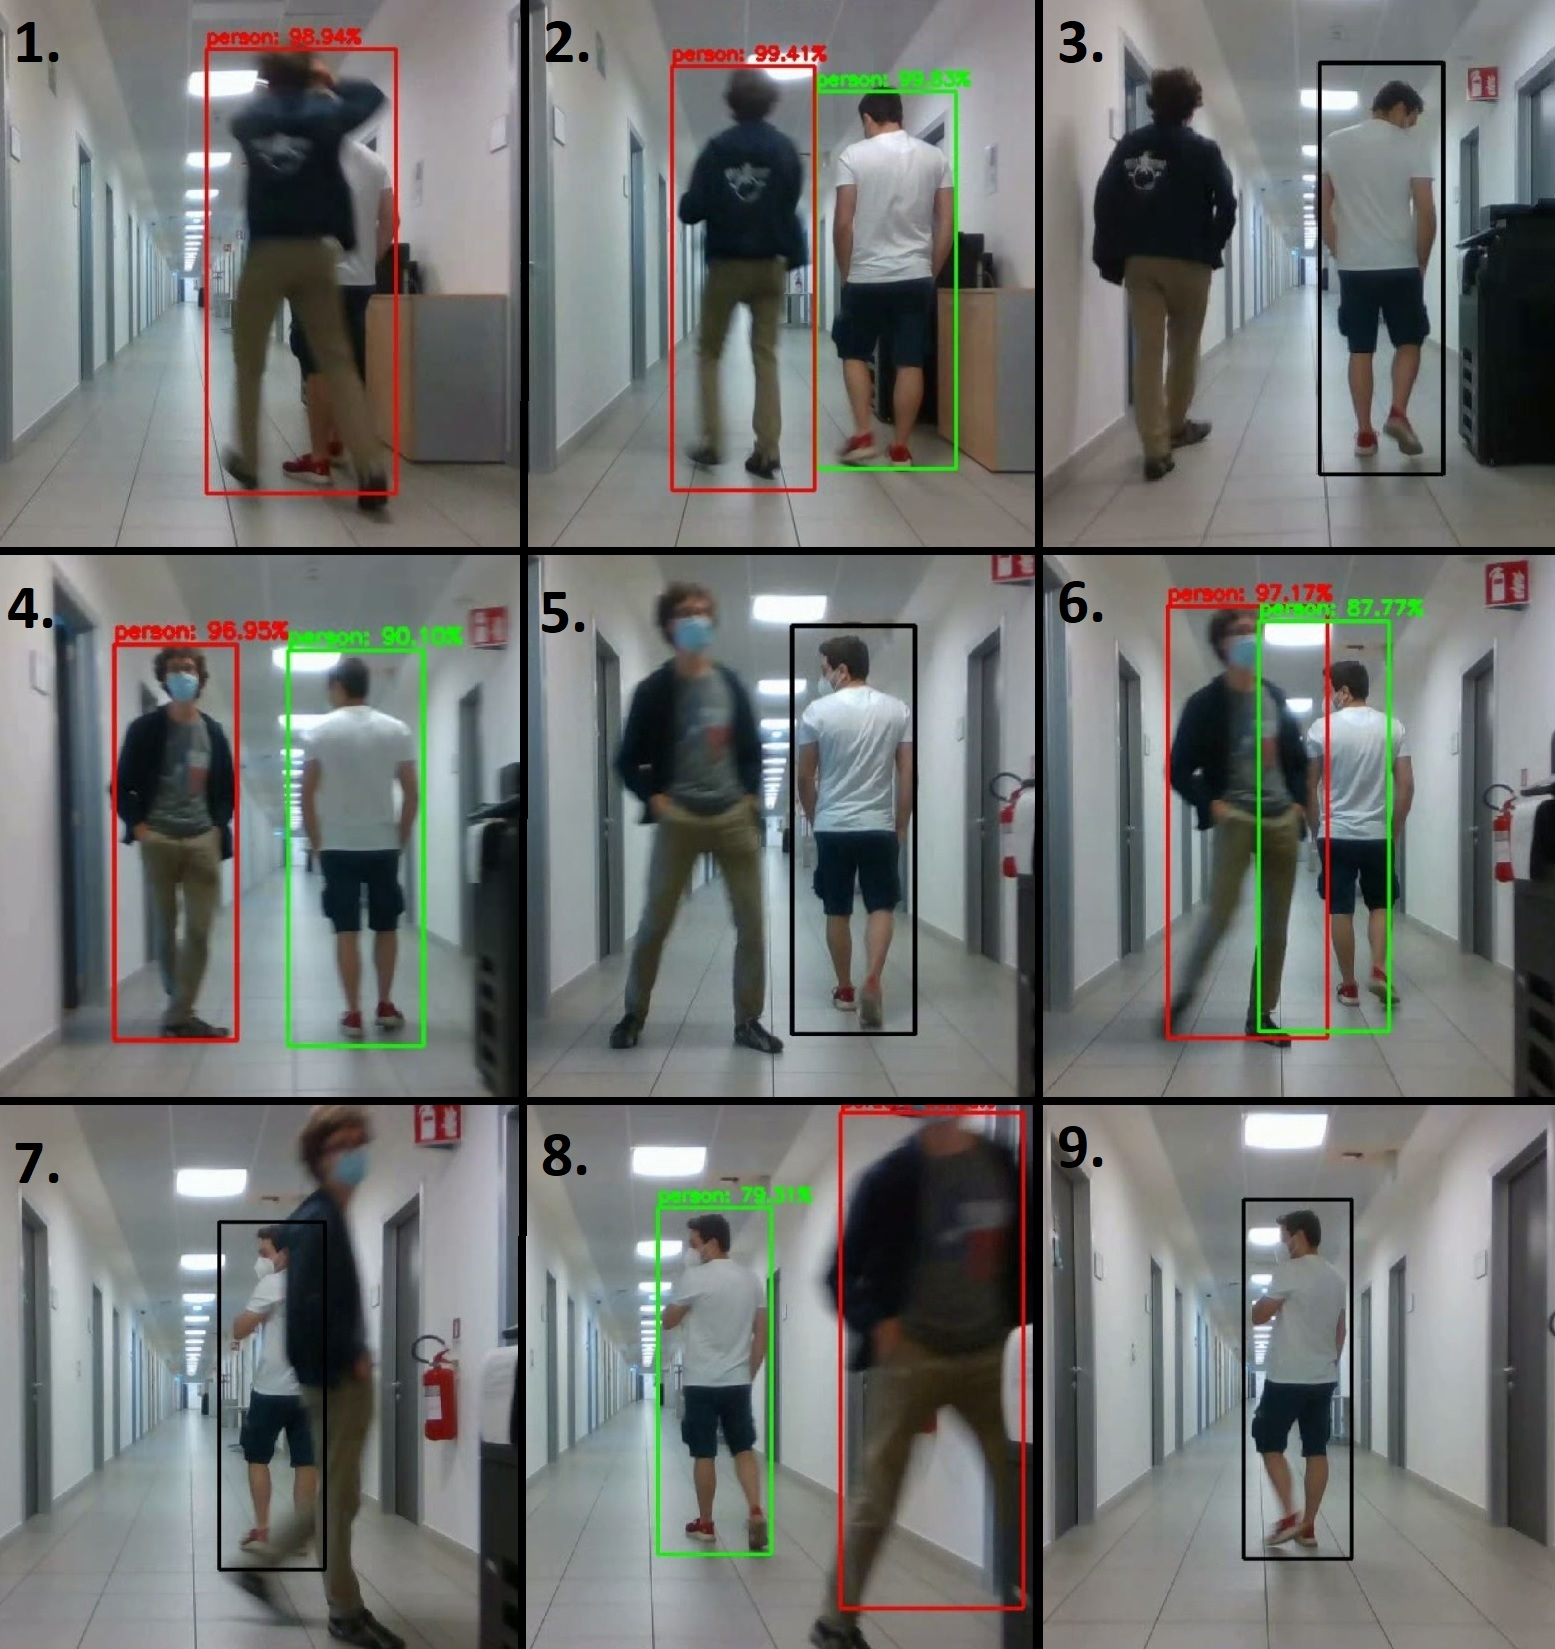
\includegraphics[width=\linewidth]{images/solution/sequenceTrackOk}
	\captionsetup{margin=0.5cm}
	\caption[A video clip frames sequence of the tracking.]{A sequence of images representing a video clip while the robot is following the leader. The coloured rectangles in the images have different meanings. \textbf{\textcolor{green}{Green}} is the detection recognised as the leader. \textbf{\textcolor{red}{Red}} is a detection recognised as a not important person. \textbf{Black} is the tracker while following the leader.\\
		In this sample the leader is hidden twice and both times the algorithm is able to detect it back again and continue the tracking.}
	\label{fig:sequenceTracking}
\end{figure}


\subsection{Detection and tracking ratio} \label{sec:ratioDetectTrack}
It is fundamental to precisely define the alternation of the detection and the tracking along with the execution of the general method. This calibration is a trade-off among processing speed and localization accuracy. As shown in~\Cref{tab:detectionPerformances} and in~\Cref{tab:trackersFPS} the processing speed of the two modules is completely different. The detection is much slower compared to the tracking. Therefore, the highest FPS rate is reached with a tracker only solution, on the other hand, the highest localization accuracy is achieved with detection only technique. Note that with only detection and multiple subjects, the leader is identified thanks to the recognition module.\\
The disclaimer is to choose the minimum required FPS rate and then hope that the accuracy is enough. In our case, we have fixed $5$ FPS as a target. To respect this limit the detection is executed once every $10$ frames. It is important to remember that if a single detection fails or the leader is not found, the tracker cannot be started. Consequently, from that moment on the frames are processed with detection-only. This recover procedure run at low FPS but the leader is momentarily lost, hence, it is not important.\\
\\
If the high FPS needs to be reached the solution may consist of changing this mechanic. The detector might be started only after the tracker reports that it lost the leader. This will reduce the number of detections and improve the overall FPS rate. Unfortunately, a lot of trackers are not precisely able to recognize when the tracked subject has been lost, hence the implementation is not straightforward, and at the moment has not been written yet.


\subsection{Drift tolerance optimization} \label{sec:driftOptimization}
The idea of this optimization comes from two conditions that should be managed. On one hand, the drift problem that is one of the main weaknesses of the trackers, in fact over a long video sequence it can be a huge problem. On the other hand, the proximity assumption (\Cref{fig:challenge_proximity}) that allows the tracked subject to move only for a limited number of pixels per frame.\\
These two conditions combined can be used to wisely classify the new detections once the tracker has been stopped. If a new detection is too far away compared to the last known position of the leader, it cannot be the leader itself. Otherwise, the recognition module should be used to normally predict the class of the new bounding box.\\
We have defined the tolerance of the movement as:
$$d = t\cdot s\cdot\left(\frac{w}{100}\right)^{2}$$
In the above formula the symbols represent:
\begin{itemize}
	\item \textbf{d} is the distance allowed.
	\item \textbf{t} is the time elapsed from the last correct detection of the leader. It is used to manage the drift problem independently of the ratio between tracking and detection.
	\item \textbf{s} is an empirical scale factor, experimentally measured to be around $0.05$. It is the hyper-parameter to manage this optimization. 
	\item \textbf{w} is the width of the last bounding box during the tracking. It is used to simulate the distance of the leader from the camera. Compared to a far detection, a close leader has a bigger bounding box hence the multiplying factor is greater. This difference is fundamental to manage the fast 2D movement of a close subject.
\end{itemize}
In~\Cref{fig:driftOptimizationFail} is shown an example where a person is immediately classified as negative because it is too far away. Instead, in~\Cref{fig:driftOptimizationOk} the person is inside the tolerance and further analysis with KNN has classified this person as the leader.

\begin{figure}[!h]
	\centering
	\begin{subfigure}[!h]{0.49\textwidth}
		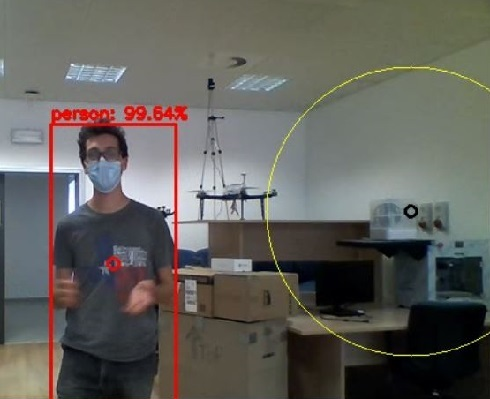
\includegraphics[width=\linewidth]{images/solution/driftOptimizationFail}
		\captionsetup{margin=0.5cm}
		\caption{The person is classified as Negative because it is outside of the \textit{drift tolerance} circle.}
		\label{fig:driftOptimizationFail}
	\end{subfigure}
	\begin{subfigure}[!h]{0.39\textwidth}
		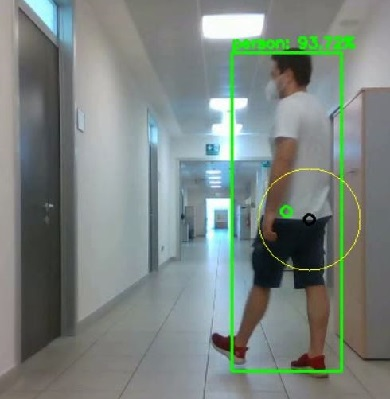
\includegraphics[width=\linewidth]{images/solution/driftOptimizationOk}
		\caption{The person is classified as Positive because it is outside of the \textit{drift tolerance} circle.}
		\label{fig:driftOptimizationOk}
	\end{subfigure}
	\captionsetup{margin=1.4cm}
	\caption[Two samples of the \textit{drift tolerance} optimization.]{Two samples of the \textit{drift tolerance} optimization represented as a \textbf{\textcolor{orange}{yellow}} circle, centred on the last known position (a small \textbf{black} circle).}
	\label{fig:driftOptimization}
\end{figure}

\subsection{Multiple leaders corner case} \label{sec:multipleleaders}
It may happen that there are two people both inside the \textit{drift tolerance} circle and both are classified as the leader from KNN. This of course is real scenario impossible (a person cannot be duplicated) hence only one can be chosen as the right one. Further analysis can be used but we have chosen a simpler idea: \textit{"The closest subject to the last know position will be the official leader"}.\\
In~\Cref{fig:leaderSubjectDoubleMatch} there is a sample scenario registered before the introduction of this elaboration.
\begin{figure}[!h]
	\centering
	\begin{subfigure}[!h]{0.49\textwidth}
		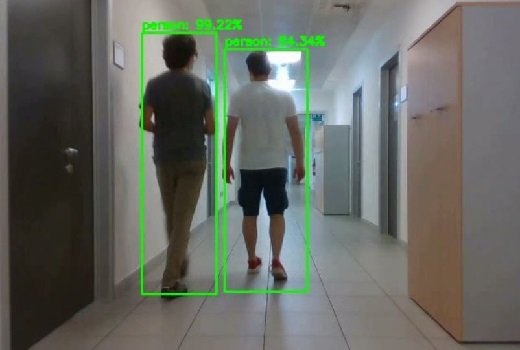
\includegraphics[width=1\linewidth]{images/solution/leaderSubjectDoubleMatch}
		\captionsetup{margin=0.2cm}
		\caption{Two recognised leader, instead one detection is a random person.}
		\label{fig:leaderSubjectDoubleMatch}
	\end{subfigure}
	\begin{subfigure}[!h]{0.49\textwidth}
		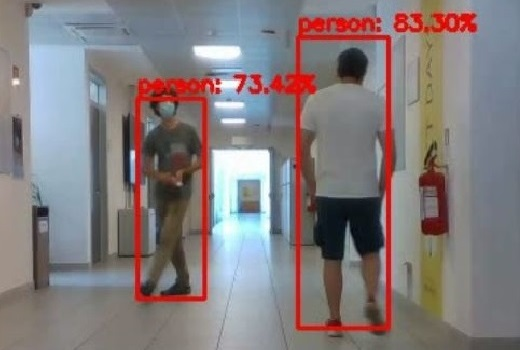
\includegraphics[width=1\linewidth]{images/solution/leaderSubjectDoubleFail}
		\captionsetup{margin=0.2cm}
		\caption{Two recognised random people, instead one detection is the leader.}
		\label{fig:leaderSubjectDoubleFail}
	\end{subfigure}
	\captionsetup{margin=0.5cm}
	\caption{Two failed scenarios where the two people are wrongly recognised.}
	\label{fig:qqq}
\end{figure}

\subsection{KNN tolerance against false-negative} \label{sec:knnToleranceToFN}
The previous section introduces the failure of the KNN classifier that predicts a leader in exceed. This is a false-positive classification. As explained this is miss prediction can be managed. On the other hand, a false-negative classification is a much bigger problem. It happens when the leader is classified as negative, an example is shown in~\Cref{fig:leaderSubjectDoubleFail}.\\
This wrong prediction is complex because, after the classification, the generated representative point and its new label are fed into KNN. This false-negative represent a point wrongly classified. However, also a false-positive is fed into KNN but if there are multiple leaders further analysis can reduce them. Instead, a leader classified as negative cannot be re-evaluated hence it cannot be converted into a correct prediction, it will be an error forever.\\
Due to the mechanics of KNN, a small set of wrong classified points can cause a lot of wrong classifications in future analysis. Therefore we absolutely want to avoid false-negative predictions.